%UCS-1: Analisi dei risultati

\begin{figure}
\centering
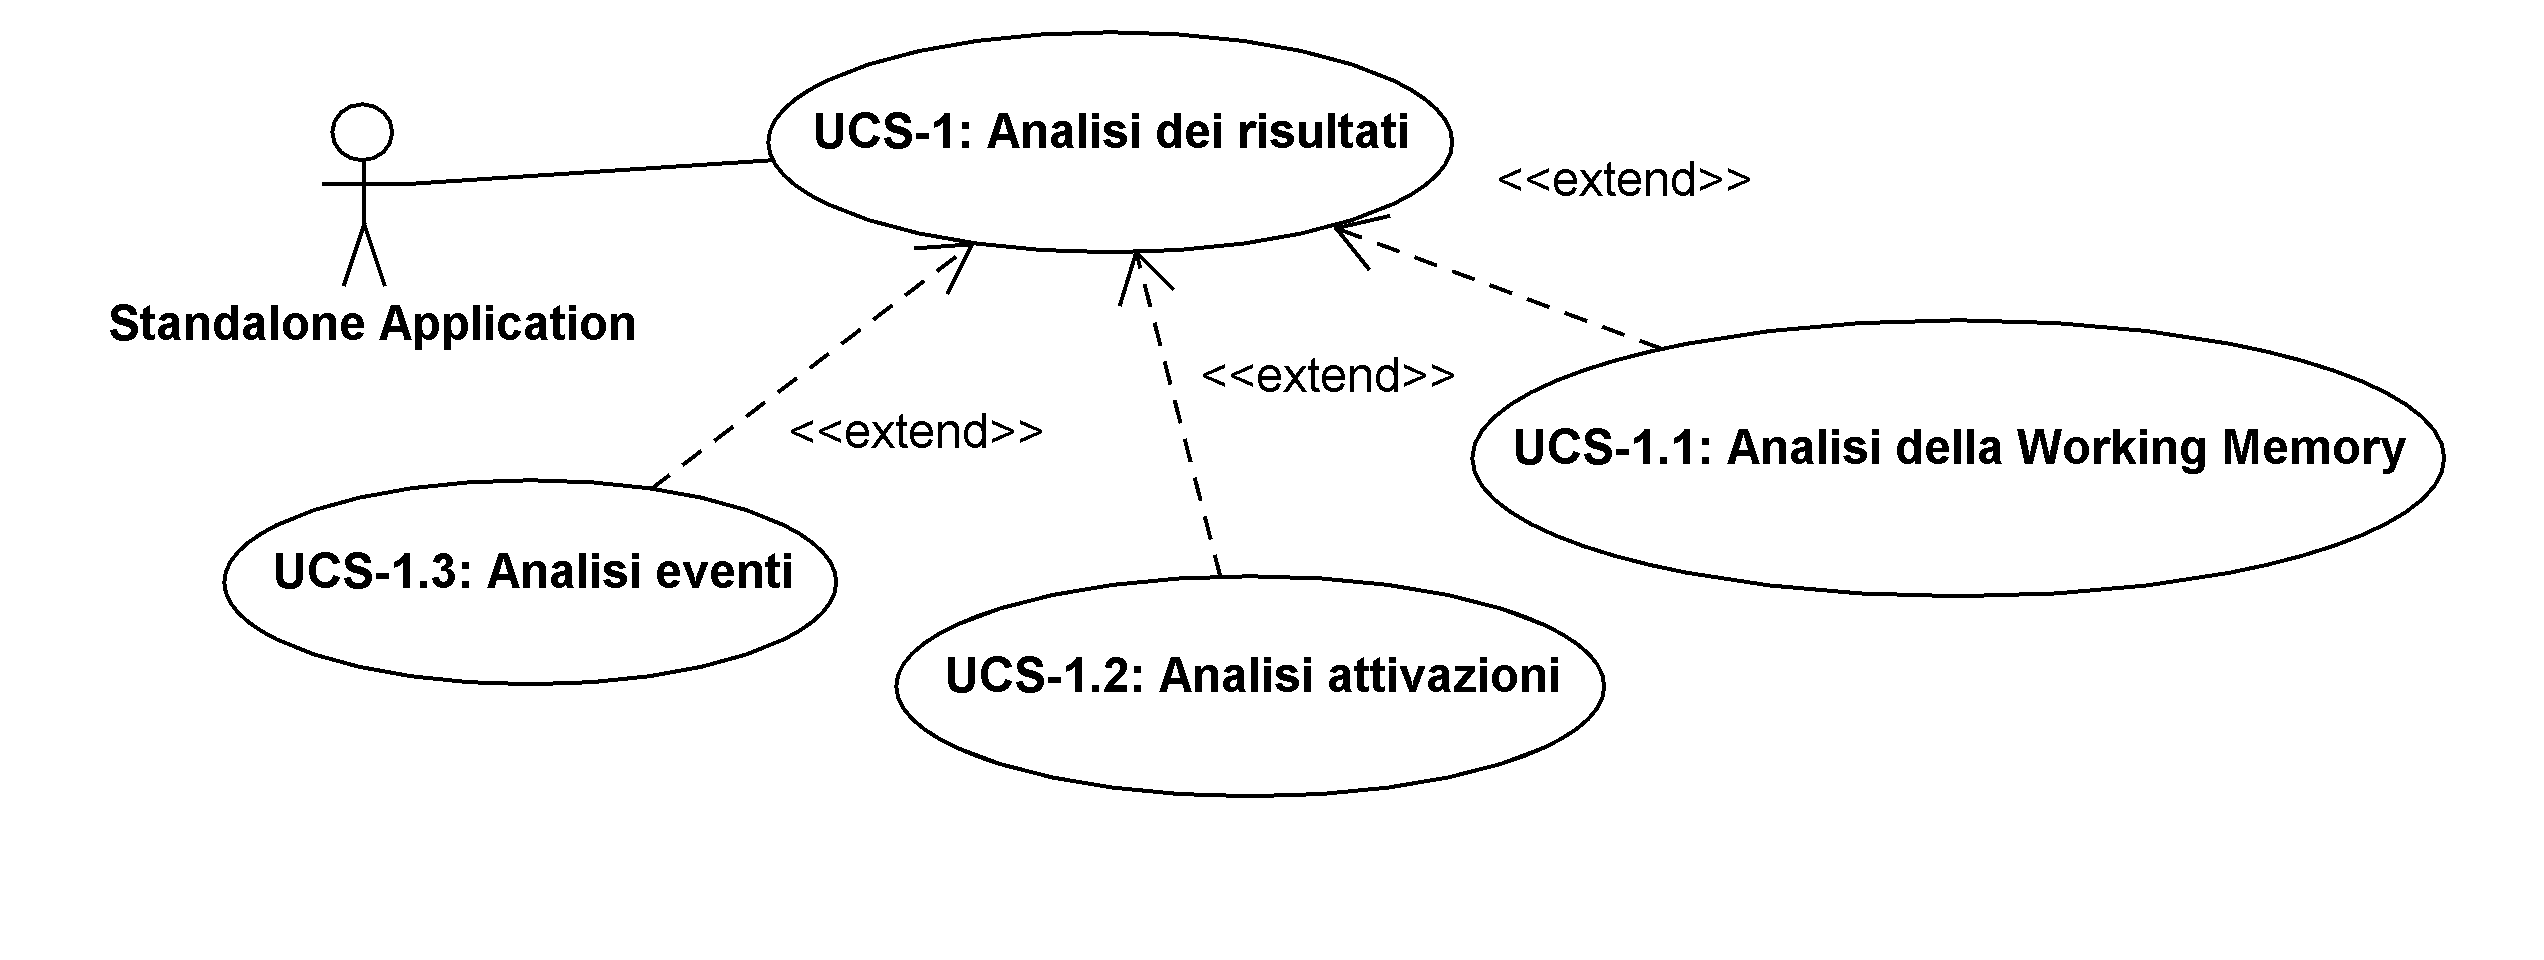
\includegraphics[width=1.1\textwidth]{Immagini/Capitolo2/UseCases/UCS-1.png}
\caption{Diagramma dei casi d'uso UCS-1}\label{fig:uc-ucs-1}
\end{figure}

\begin{itemize}
	\item \textbf{Attori:} Standalone Application
	\item \textbf{Scopo e descrizione:} la Standalone Application deve avere la possibilità di accedere alle informazioni riguardanti lo stato finale di un'elaborazione eseguita dal software e ricevere notifica del verificarsi di eventi durante l'elaborazione
	\item \textbf{Pre-condizioni:} la Standalone Application ha eseguito con successo il caso d'uso \emph{UCC-1.2}
	\item \textbf{Post-condizioni:} la Standalone Application ha ottenuto le informazioni necessarie
	\item \textbf{Flusso principale degli eventi:}
		\begin{enumerate}
			\item la Standalone Application richiede informazioni sullo stato terminale di elaborazione del software
				\begin{itemize}
					\item la Standalone Application richiede informazioni sullo stato della \emph{working-memory} (si guardi il caso d'uso \emph{UCS-1.1})
					\item la Standalone Application richiede informazioni sullo stato delle attivazioni ancora presenti (si guardi il caso d'uso \emph{UCS-1.2})
					\item la Standalone Application valuta il verificarsi di un evento (si guardi il caso d'uso \emph{UCS-1.3})
				\end{itemize}
			\item la Standalone Application ottiene le informazioni richieste
		\end{enumerate}
\end{itemize}


\paragraph{UCS-1.1: Analisi della Working-Memory}

\begin{itemize}
	\item \textbf{Attori:} Standalone Application
	\item \textbf{Scopo e descrizione:} la Standalone Application deve avere accesso alle informazioni presenti nella \emph{Working Memory}
	\item \textbf{Pre-condizioni:} la Standalone Application ha eseguito con successo il caso d'uso \emph{UCC-1.2}
	\item \textbf{Post-condizioni:} la Standalone Application ottiene le informazioni sui fatti presenti nella \emph{Working Memory}
	\item \textbf{Flusso principale degli eventi:}
		\begin{enumerate}
			\item la Standalone Application richiede una vista dei dati presenti nella \emph{Working Memory}
				\begin{itemize}
					\item la Standalone Application può limitare la ricerca solo ai fatti relativi ad un sottogruppo dei moduli specificati
					\item la Standalone Application può richiedere tutti i fatti presenti nella \emph{Working Memory}
				\end{itemize}
			\item la Standalone Application ottiene l'elenco dei fatti richiesti
		\end{enumerate}
\end{itemize}


\paragraph{UCS-1.2: Analisi attivazioni}

\begin{itemize}
	\item \textbf{Attori:} Standalone Application
	\item \textbf{Scopo e descrizione:} la Standalone Application deve avere accesso alle informazioni presenti nell'agenda delle attivazioni
	\item \textbf{Pre-condizioni:} la Standalone Application ha eseguito con successo il caso d'uso \emph{UCC-1.1}
	\item \textbf{Post-condizioni:} la Standalone Application ottiene l'elenco di attivazioni disponibili nell'agenda delle attivazioni nelle modalità che ha indicato
	\item \textbf{Flusso principale degli eventi:}
		\begin{enumerate}
			\item la Standalone Application richiede una vista sulle attivazioni presenti nell'agenda delle attivazioni.
				\begin{itemize}
					\item la Standalone Application può limitare la ricerca solo alle attivazioni relative ad un sottogruppo dei moduli specificati
					\item la Standalone Application può richiedere l'intera lista delle attivazioni presenti in agenda
				\end{itemize}
			\item la Standalone Application ottiene l'elenco delle attivazioni richieste
		\end{enumerate}
\end{itemize}


\paragraph{UCS-1.3: Analisi eventi}

\begin{itemize}
	\item \textbf{Attori:} Standalone Application
	\item \textbf{Scopo e descrizione:} la Standalone Application deve ricevere notifica del verificarsi di un evento per il quale ha espresso interesse nelle modalità previste dal software
	\item \textbf{Pre-condizioni:} la Standalone Application ha eseguito con successo il caso d'uso \emph{UCC-1.2.3}
	\item \textbf{Post-condizioni:} la Standalone Application ha eseguito il comportamento associato ad un determinato evento
	\item \textbf{Flusso principale degli eventi:}
		\begin{enumerate}
			\item la Standalone Application esprime interesse relativamente al verificarsi di un evento (si guardi caso d'uso \emph{UCC-1.2.3})
			\item la Standalone Application osserva la notifica del verificarsi di un evento
			\item la Standalone Application analizza i parametri relativi all'evento
			\item la Standalone Application esegue il comportamento associato all'evento con i parametri forniti
		\end{enumerate}
\end{itemize}





